\documentclass[pdf]{beamer}
\usepackage{minted}
\setminted{encoding=utf-8}
\usemintedstyle{colorful}
\usepackage{fontspec}
\usepackage{etoolbox}
\AtBeginEnvironment{minted}{\fontsize{8}{8}\selectfont}
\usepackage{amsmath}
\usepackage{amsfonts}
\usepackage{amssymb}
\usepackage{graphicx}
\usepackage{subfigure}
\usepackage{outlines}
\usepackage{hyperref}
\mode<presentation>{\usetheme{}}
\title{Why Types Matter}
%% \subtitle{}
\author{Slavomir Kaslev \\
  \href{mailto:slavomir.kaslev@gmail.com}{slavomir.kaslev@gmail.com}}

\begin{document}

\begin{frame}
  \titlepage
\end{frame}

\begin{frame}{QOTD}
  ``Bad programmers worry about the code. Good programmers worry about data structures and their relationships.'' \mbox{Linus Torvalds}
\end{frame}

\begin{frame}{Introduction}
  \begin{outline}
    \1 Types were first proposed by Bertrand Russell in 1902 to resolve Russell's paradox in Gottlob Frege's naive set theory
    \pause
    \1 Since then types have been studied on their own and combined with Alonzo Church's $\lambda$-calculus
    provide the theoretical framework of modern functional languages
    \pause
    \1 There are quite a few different flavors of type theories around
    \pause
    \2 Simply typed lambda calculus (1940s), System F (1970s)
    \3 Haskell, OCaml, ML, ...
    \pause
    \2 Martin-Löf Dependent Type Theory (1970s)
    \3 Agda, Coq, Idris, Lean, ..
    \pause
    \2 Homotopy Type Theory (2000s)
    \pause
    \2 ...
    \pause
    \1 Today, while the OOP world is catching up with functional programming, Haskell is catching up with dependent types
  \end{outline}
\end{frame}

\begin{frame}{The Levels}
  \begin{center}
    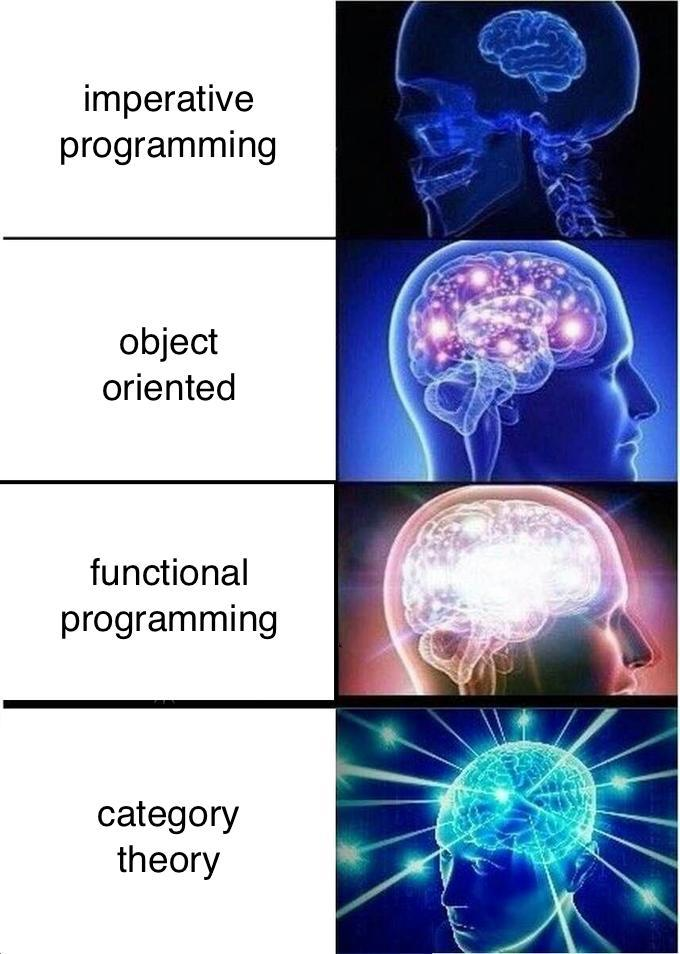
\includegraphics[scale=0.23]{images/levels}
  \end{center}
\end{frame}

\begin{frame}{What are Types}
  \begin{outline}
    \1 Roughly speaking, types are specification of their possible values
    \pause
    \1 In typed programming languages each value $a$ has a type $A$ and we'll denote this as $a : A$
    \pause
    \1 Instead of trying to define precisely what types are let's see what we can do with them
    \pause
    \1 For one, given the types $A : Type$ and $B : Type$ one can construct say $A \to B$, the type of functions from $A$ to $B$
    \pause
    \1 ($\lambda (x : Int) \mapsto x + 1) : Int \to Int$
  \end{outline}
\end{frame}

\begin{frame}{Algebraic Data Types}
  \begin{outline}
    \pause
    \1 The idea of algebraic data types is to introduce the operations $\oplus$ and $\otimes$ that
    given the types $A : Type$ and $B : Type$ construct new types namely:
    \pause
    \2 $A \oplus B$, disjoint union of $A$ and $B$
    \pause
    \2 $A \otimes B$, product of $A$ and $B$
  \end{outline}
\end{frame}

\begin{frame}[fragile]{$A \otimes B$: Type product in Haskell}
  \begin{minted}[escapeinside=~~,mathescape=true]{Haskell}
    data Pair = MkPair Int String
    -- MkPair :: Int -> String -> Pair
  \end{minted}
  \pause
  \begin{minted}[escapeinside=~~,mathescape=true]{Haskell}
    data R3 = MkR3 Float Float Float
    -- MkR3 :: Float -> Float -> Float -> R3
  \end{minted}
  \pause
  \begin{minted}[escapeinside=~~,mathescape=true]{Haskell}
    data One = MkOne
    -- MkOne :: One
  \end{minted}
  \pause
  \begin{minted}[escapeinside=~~,mathescape=true]{Haskell}
    data B x = B x x
    -- B :: x -> x -> B x
  \end{minted}
\end{frame}

\begin{frame}[fragile]{$A \oplus B$: Disjoint union in Haskell}
  \begin{minted}[escapeinside=~~,mathescape=true]{Haskell}
    data Bool = True | False
    -- True, False :: Bool
  \end{minted}
  \pause
  \begin{minted}[escapeinside=~~,mathescape=true]{Haskell}
    data Maybe x = Nothing | Some x
    -- Nothing :: Maybe x
    -- Some :: x -> Maybe x
  \end{minted}
  \pause
  \begin{minted}[escapeinside=~~,mathescape=true]{Haskell}
    data List x = Nil | Cons x (List x)
    -- Nil :: List x
    -- Cons :: x -> List x -> List x
  \end{minted}
  \pause
  \begin{minted}[escapeinside=~~,mathescape=true]{Haskell}
    data BinTree x = Leaf x | Branch (BinTree x) (BinTree x)
    -- Leaf :: x -> BinTree x
    -- Branch :: BinTree x -> BinTree x -> BinTree x
  \end{minted}
\end{frame}

\begin{frame}{Analytic Combinatorics}
  \begin{outline}
    \1 Analytic combinatorics deals with counting combinatorial objects by means of their generating functions
    \pause
    \2 See the book ``Analytic Combinatorics'' by Philippe Flajolet and Robert Sedgewick for an in-depth introduction
    \pause
    \1 What is a generating function?
    \pause
    \1 Given a combinatorial class $A$ and a size function $w : A \to \mathbb{N}$ we define $A$'s ordinary generating function (OGF) as
    \begin{align*}
      A(x) = \sum_{a : A}{x^{w(a)}} = \sum_{n=0}^{\infty}{a_n x^n}
    \end{align*}
    \pause
    \1 The numbers $a_n$ tell us how many objects in $A$ are of size $n$
  \end{outline}
\end{frame}

\begin{frame}[fragile]{Symbolic Method: Finding generating functions}
  \begin{outline}
    \1 Flajolet and Sedgewick propose a simple method of finding equation for the OGF of a given combinatorial construction expressed in their specification language
    \pause
    \1 In the special case of algebraic data types, the symbolic method uses the fact that if $A, B, C$ are types and $A(x), B(x), C(x)$ are the corresponding OGFs then
    \begin{align*}
      C = A \oplus B &\implies C(x) = A(x) + B(x) \\
    \text{and} \\
      C = A \otimes B &\implies C(x) = A(x) B(x)
    \end{align*}
    \pause
    \1 For example
    \begin{minted}[escapeinside=~~,mathescape=true]{Haskell}
      data Foo x = F0 | F1 x | F2 x (Foo x)
    \end{minted}
    \pause
    \begin{align*}
      Foo(x) = 1 + x + x Foo(x)
    \end{align*}
  \end{outline}
\end{frame}

\begin{frame}[fragile]{Symbolic Method: Examples}
  \begin{minted}[escapeinside=~~,mathescape=true]{Haskell}
    data Empty
  \end{minted}
  \pause
  \begin{align*}
    E(x) &= 0
  \end{align*}

  \pause
  \begin{minted}[escapeinside=~~,mathescape=true]{Haskell}
    data One = One
  \end{minted}
  \pause
  \begin{align*}
    O(x) &= 1
  \end{align*}

  \pause
  \begin{minted}[escapeinside=~~,mathescape=true]{Haskell}
    data Bool = True | False
  \end{minted}
  \pause
  \begin{align*}
    B(x) &= 1 + 1
  \end{align*}
  \pause
  \begin{align*}
    B(x) &= 2
  \end{align*}
\end{frame}

\begin{frame}[fragile]{Symbolic Method: Examples}
  \begin{minted}[escapeinside=~~,mathescape=true]{Haskell}
    data Maybe x = None | Just x
  \end{minted}
  \pause
  \begin{align*}
    M(x) &= 1 + x
  \end{align*}

  \pause
  \begin{minted}[escapeinside=~~,mathescape=true]{Haskell}
    data L x = Nil | Cons x (L x)
  \end{minted}
  \pause
  \begin{align*}
    L(x) &= 1 + x L(x)
  \end{align*}
  \pause
  \begin{align*}
    L(x) &= \frac{1}{1-x}
  \end{align*}
  \pause
  \begin{align*}
    L(x) &= 1 + x + x^2 + x^3 + x^4 + x^5 + x^6 + x^7 +...
  \end{align*}
\end{frame}

\begin{frame}[fragile]{Symbolic Method: Examples}
  \begin{minted}[escapeinside=~~,mathescape=true]{Haskell}
    data T x = Leaf x | Branch (T x) (T x)
  \end{minted}
  \pause
  \begin{align*}
    T(x) &= x + T^2(x)
  \end{align*}
  \pause
  \begin{align*}
    T(x) &= \frac{1 \pm \sqrt{1 - 4 x}}{2}
  \end{align*}
  \pause
  \begin{align*}
    T(x) &= x + x^2 + 2 x^3 + 5 x^4 + 14 x^5 + 42 x^6 + 132 x^7 +...
  \end{align*}
\end{frame}

\begin{frame}[fragile]{Symbolic Method: Examples}
  \begin{minted}[escapeinside=~~,mathescape=true]{Haskell}
    data B x = B0 x | B1 x
    data L x = Nil | Cons x (L x)
    data Bits x = Bits (L (B x))
  \end{minted}
  \pause
  \begin{align*}
    B(x) &= 2 x \\
    L(x) &= 1 + x L(x) \\
    Bits(x) &= L(B(x))
  \end{align*}
  \pause
  \begin{align*}
    Bits(x) &= \frac{1}{1 - 2x}
  \end{align*}
  \pause
  \begin{align*}
    Bits(x) &= 1 + 2 x + 4 x^2 + 8 x^3 + 16 x^4 + 32 x^5 + 64 x^6 + 128 x^7 +...
  \end{align*}
\end{frame}

\begin{frame}[fragile]{Symbolic Method: Examples}
  \begin{minted}[escapeinside=~~,mathescape=true]{Haskell}
    data C x = C0 x | C1 x x
    data L x = Nil | Cons x (L x)
    data H = H0 (L (C x))
  \end{minted}
  \pause
  \begin{align*}
    C(x) &= x + x^2 \\
    L(x) &= 1 + x L(x) \\
    H(x) &= L(C(x))
  \end{align*}
  \pause
  \begin{align*}
    H(x) &= \frac{1}{1 - x - x^2}
  \end{align*}
  \pause
  \begin{align*}
    H(x) &= 1 + x + 2 x^2 + 3 x^3 + 5 x^4 + 8 x^5 + 13 x^6 + 21 x^7 +...
  \end{align*}
\end{frame}

\begin{frame}[fragile]{Symbolic Method: Examples}
  \begin{minted}[escapeinside=~~,mathescape=true]{Haskell}
    data F x = F0 x | F1 (F (G x))
    data G x = G0 x | G1 x (G x)
  \end{minted}
  \pause
  \begin{align*}
    f(x) &= x + f(g(x)) \\
    g(x) &= x + x g(x)
  \end{align*}
  \pause
  \begin{align*}
    f(x) &= x + f(\frac{x}{1-x})
  \end{align*}
  \pause
  \begin{align*}
    f(x) &= \sum_{n=0}^{\infty} \frac{x}{1-n x}
  \end{align*}
  \pause
  \begin{align*}
    f(x) &= \psi(-\frac{1}{x}) + \gamma \\
    \psi(x) &= \frac{d}{dx}\ln\Gamma(x) = \frac{\Gamma'(x)}{\Gamma(x)}
  \end{align*}
\end{frame}

\begin{frame}{Curry–Howard correspondence: Propositions as types}
  \begin{outline}
    \1 The Curry–Howard correspondence is an observation that two seemingly unrelated formalism, namely typed $\lambda$-calculus and proof theory, are in fact closely related
    \pause
    \1 The general idea is that one can interpret a type $A$ as a proposition in proof theory
    \pause
    \1 And a value $a : A$ of type $A$ is interpreted as a proof of the corresponding proposition
    \pause
    \1 The function type $A \to B$ gets interpreted as the proposition $A \implies B$
    \pause
    \1 The types $A \oplus B$ and $A \otimes B$ get interpreted as $A \lor B$ and $A \land B$
  \end{outline}
\end{frame}

\begin{frame}{The Rosetta Stone}
  \begin{center}
    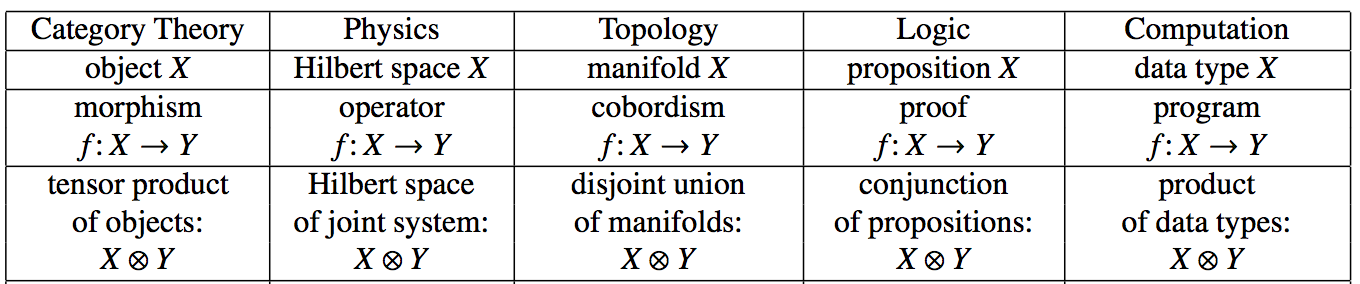
\includegraphics[scale=0.47]{images/rosetta}
  \end{center}
\end{frame}

\begin{frame}{The Rosetta Stone: Homotopy Type Theory style}
  \begin{center}
    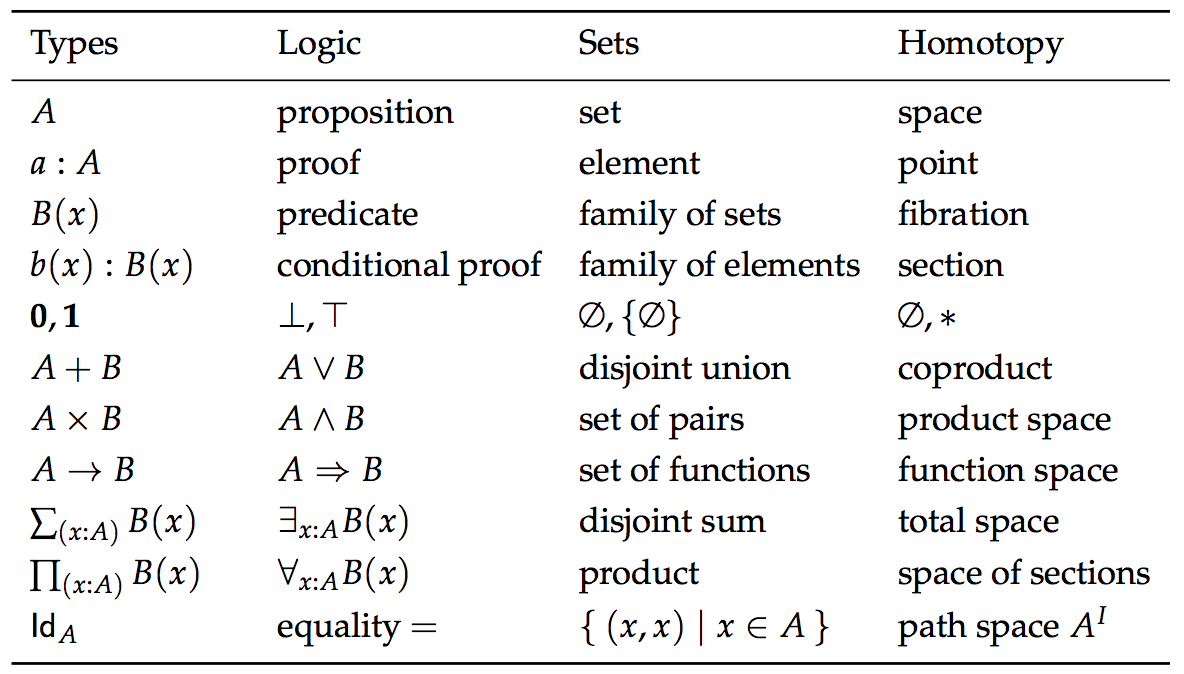
\includegraphics[scale=0.47]{images/hott}
  \end{center}
\end{frame}

\begin{frame}{Dependent Types}
  \begin{outline}
    \1 The idea of dependent types is to allow types to depend on values
    \pause
    \1 In simply typed $\lambda$-calculus values and types are separate
    \pause
    \1 In Haskell's core language, for example, values and types get mapped to two separate data structures: \mintinline{Haskell}{data Expr} and \mintinline{Haskell}{data Type} respectively
    \pause
    \1 In dependently typed languages those two are unified
    \pause
    \1 The core language consist of a single data structure: \mintinline{Haskell}{data Expr} that represents both values and types
  \end{outline}
\end{frame}

\begin{frame}{Dependent Types II}
  \begin{outline}
    \1 To allow values to appear at the type level, the function type $A \to B$ and the product type $A \otimes B$ get generalized to $\Pi$-types and $\Sigma$-types respectively
    \pause
    \1 $\prod_{a : A}{B(a)}$ is analogous to the $\forall$ quantifier $\forall a : A, B(a)$ in logic
    \1 $\sum_{a : A}{B(a)}$ is analogous to the $\exists$ quantifier $\exists a : A, B(a)$ in logic
    \pause
    \1 The last ingredient is the equality type $Id_{A} : A \to A \to Type$ populated by proofs $a =_{A} b : Id_{A}(a, b)$
  \end{outline}
\end{frame}

\begin{frame}{Dependent Types: Examples}
  \pause
  \begin{align*}
    \prod_{a : \mathbb{N}} \prod_{b: \mathbb{N}} (a \leq b \to \sum_{n:\mathbb{N}} a + n =_{\mathbb{N}} b)
  \end{align*}
  \pause
  \begin{align*}
    Iso(A, B : Type) := \sum_{f : A \to B}\sum_{g : B \to A} (\prod_{a : A}{g(f(a)) =_{A} a}) \otimes (\prod_{b : B}{f(g(b)) =_{B} b})
  \end{align*}
  \begin{outline}
  \end{outline}
\end{frame}

\begin{frame}{Challenge}
  \begin{outline}
    \1 ``Learn a new programming language every year'' from the book ``The Pragmatic Programmer''
    \pause
    \1 ``A language that doesn't affect the way you think about programming, is not worth knowing.'' Alan Perlis
    \pause
    \1 Make the next language you'll learn be dependently typed
    \pause
    \2 Lean, lead by the author of the Z3 Theorem Prover
    \pause
    \2 Idris
    \pause
    \2 Agda
    \pause
    \2 Coq
  \end{outline}
\end{frame}

\begin{frame}[fragile]{A taste of Lean}
  \begin{minted}[escapeinside=@@,mathescape=true]{Lean}
theorem prod_commutative (p q : Type) : p × q → q × p :=
@$\lambda$@ hpq : p × q, prod.mk (prod.snd hpq) (prod.fst hpq)

theorem prod_commutative2 (p q : Type) : p × q → q × p :=
assume hpq : p × q,
have hp : p, from prod.fst hpq,
have hq : q, from prod.snd hpq,
show q × p, from prod.mk hq hp

theorem mul_cancel_left_or {a b c : @$\mathbb{Z}$@} (H : a * b = a * c) : a = 0 @$\lor$@ b = c :=
have H2 : a * (b - c) = 0, by simp,
have H3 : a = 0 @$\lor$@ b - c = 0, from mul_eq_zero H2,
or.imp_or_right H3 (assume H4 : b - c = 0, sub_eq_zero H4)
  \end{minted}
\end{frame}

\begin{frame}[fragile]{Set theory Lean}
  \begin{minted}[escapeinside=@@,mathescape=true]{Lean}
def set (@$\alpha$@ : Type) := @$\alpha$@ → Prop

def mem (a : @$\alpha$@) (s : set @$\alpha$@) := s a

def union (@$s_1$@ @$s_2$@ : set @$\alpha$@) : set @$\alpha$@ :=
{a | a @$\in s_1$@ @$\lor$@ a @$\in s_2$@}

def image (f : @$\alpha$@ → @$\beta$@) (s : set @$\alpha$@) : set @$\beta$@ :=
{b | @$\exists$@ a, a @$\in$@ s @$\land$@ f a = b}
  \end{minted}
\end{frame}

\begin{frame}{Further reading}
  \small
  \begin{outline}
    \1 ``Analytic Combinatorics'' by \mbox{Philippe Flajolet} and \mbox{Robert Sedgewick}
    \1 ``Physics, Topology, Logic and Computation: A Rosetta Stone'' by \mbox{John Baez} and \mbox{Mike Stay}
    \1 ``Homotopy Type Theory: Univalent Foundations of Mathematics'' by \mbox{The Univalent Foundations Program}
    \1 ``Proofs and Types'' by \mbox{Jean-Yves Girard}
    \1 ``Constructive Mathematics and Computer Programming'' by \mbox{Per Martin-L\"{o}f}
    \1 ``Tutorial: Theorem Proving in Lean'' \href{url}{https://leanprover.github.io/tutorial/}
  \end{outline}
\end{frame}

\begin{frame}{Questions?}
\end{frame}

\end{document}
